\section{Architecture}
\label{sec:architecture}

This section describes how the different components of the system are
composed to build a coherent piece. A complete diagram of the architecture can be seen in \cref{fig:architecture}. On this diagram an arrow represents an dependency. That means the pointed at component must exist for other to be complete. The diagram does not specify how that dependency is implemented. It could be a method call or some other way. A detailed description of the implementation of the different components will be described in \cref{par:implementation}.

The overall architecture is made as a layered architecture. With three main components; model, function and interface. It is set up as a closed strict architecture, which means that each layer can depend only depend on the one directly below it. Besides the three layers there is the technical platform component.

The system is separated in three subsystem: an interactive client, a presentation client and a server. The three subsystems are divided in a distributed presentation architecture. This means that the server has all the three basic layers, while the clients is only responsible displaying information given by the server. All the business logic is contained on the
server. This communication occurs through the \textit{System Interface}
components of the clients and server. The information being sent back and
forth between the clients and server is displayed in the \textit{User Interface}
component of the clients and the server.

The difference between the clients is that the interactive client, interacts by reading, writing and update the model layer on the server through the function layer, and the presentation client only reads the model, and presents for the users.

The aforementioned business logic on the server is a collection of
many different components. Each of these components have a distinct
responsibility. For example, the \textit{UserService} has the responsibility to
handle all actions related to users of the application. The
\textit{UserService} component defines the functions involving users. It is
therefore placed in the function layer of the server. To perform its
actions, the \textit{UserService} component has associations to the \textit{User}
component defined in the model layer of the server.

Another layer of the server architecture is the
technical platform. Components contained in this layer are all
libraries defined outside of the business logic of the server, but are
still as part of the complete system. For example, the
\textit{SpotifyDotNet} component is a library for streaming tracks from
Spotify. The implementation details of this is described in
\cref{cha:technicalPlatform}.
\frnote{fix pile i diagram}
\begin{figure}[H]
  \centering
  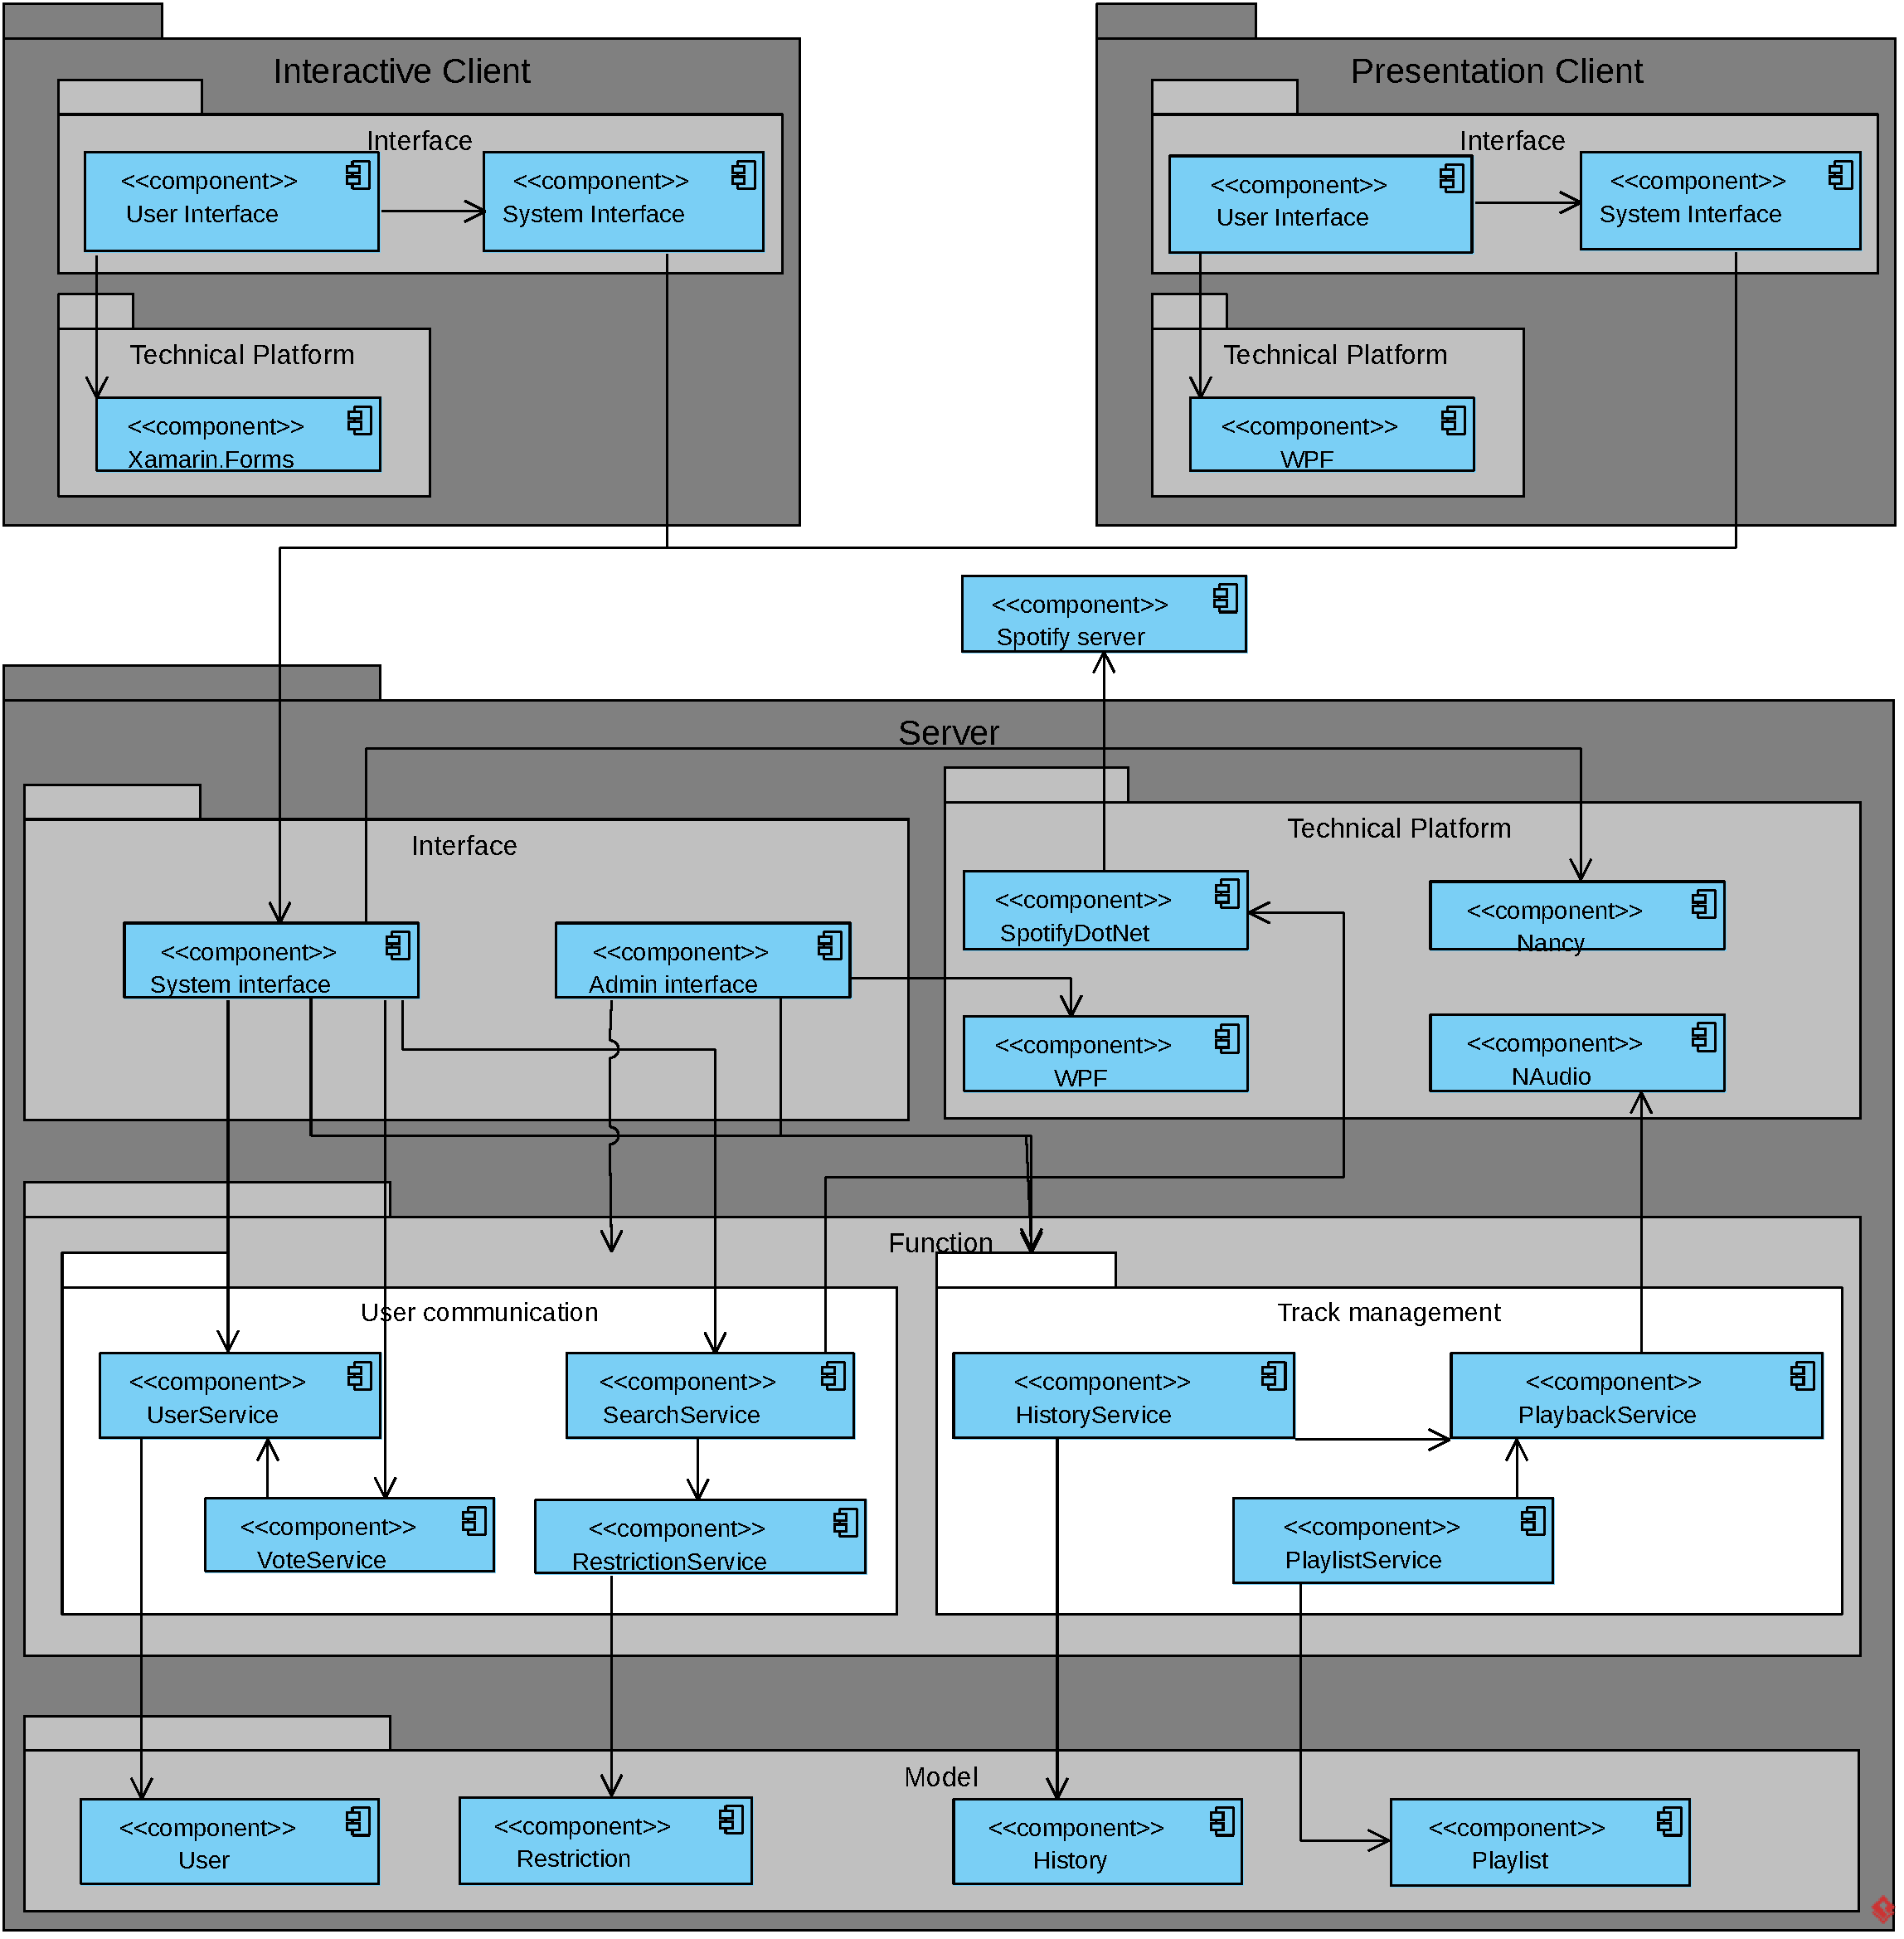
\includegraphics[width=1.2\linewidth]{Images/Arkitektur.pdf}
  \caption{Architecture of the system}\label{fig:architecture}
\end{figure}
